\documentclass[12pt,a4paper]{article}
\usepackage[a4paper, margin=0.7in]{geometry}
\usepackage{amsmath, amssymb}
\usepackage{graphicx}
\usepackage{float} % for [H] exact figure placement
\usepackage{placeins} % for \FloatBarrier
\graphicspath{{figures/}}
\usepackage{hyperref}
\usepackage{listings}
\usepackage{xcolor}
\usepackage{caption}

% Custom section numbering: a, b, c for sections, i, ii, iii for subsections
\renewcommand{\thesection}{\alph{section}}
\renewcommand{\thesubsection}{\roman{subsection}}

\lstset{
    basicstyle=\ttfamily\tiny,
    backgroundcolor=\color{gray!10},
    frame=single,
    breaklines=true,
    postbreak=\mbox{\textcolor{red}{$\hookrightarrow$}\space},
    keywordstyle=\color{blue},
    commentstyle=\color{gray},
    stringstyle=\color{orange},
    showstringspaces=false,
    columns=flexible,
    keepspaces=true,
    aboveskip=0pt,
    belowskip=0pt
}

\title{\textbf{Machine Learning Assignment Report - Week 2}}
\author{}
\date{}

% Reduce spacing
\setlength{\parskip}{0.3em}
\setlength{\floatsep}{0.2em}
\setlength{\textfloatsep}{0.2em}
\setlength{\intextsep}{0.2em}
\setlength{\topskip}{0pt}
\setlength{\topsep}{0pt}
\setlength{\partopsep}{0pt}
\setlength{\parsep}{0pt}
\setlength{\itemsep}{0pt}
\setlength{\belowdisplayskip}{0pt}
\setlength{\abovedisplayskip}{0pt}
\setlength{\belowdisplayshortskip}{0pt}
\setlength{\abovedisplayshortskip}{0pt}
\setlength{\headsep}{0pt}
\setlength{\footskip}{0pt}
\setlength{\topmargin}{0pt}
\setlength{\headheight}{0pt}
\setlength{\baselineskip}{0.9\baselineskip}

\begin{document}

\maketitle

\begin{center}
Name: Sayan Mondal\\
Student ID: 24377372\\
Strand: Future Networked Systems\\
Course: MSc. Computer Science
\end{center}

\vspace{1em}

\section*{Dataset Information}

This report uses the dataset \texttt{week2.csv} downloaded individually as required. The dataset begins with this ID line \texttt{\# id:5-5-5}.  The data has two input features \( X_1, X_2 \) and a target \( y \) which is either $-1$ or $+1$ with 1000 samples and a balanced class split.

The first two columns are the input features X1 and X2 in the dataset structure and the third column contains the target values y. The total number of samples is 1000 data points with an equal distribution of 500 samples for each class (+1 and -1).

\section{Logistic Regression}

\subsection{Data Visualization}

I used a 2D scatter plot (using matplotlib) to plot the training data where X1 is on the x-axis and X2 on the axis y. Both the data points use distinct markers, blue '+' mark represents class +1 and green 'o' markers represent class -1 in the same plot.

\begin{lstlisting}[language=Python, caption={Data Visualization}]
plt.figure(figsize=(10, 6))
plt.scatter(X1[y==1], X2[y==1], marker='+', color='blue', s=50, label="Class +1")
plt.scatter(X1[y==-1], X2[y==-1], marker='o', color='green', s=50, label="Class -1")
plt.xlabel("X1")
plt.ylabel("X2")
plt.title("(a)(i) Data Visualization")
plt.legend()
plt.grid(True, alpha=0.3)
plt.show()
\end{lstlisting}

The data appears linearly separable with some overlaps between classes, making a linear decision boundary effective for most points.

\begin{figure}[H]
    \centering
    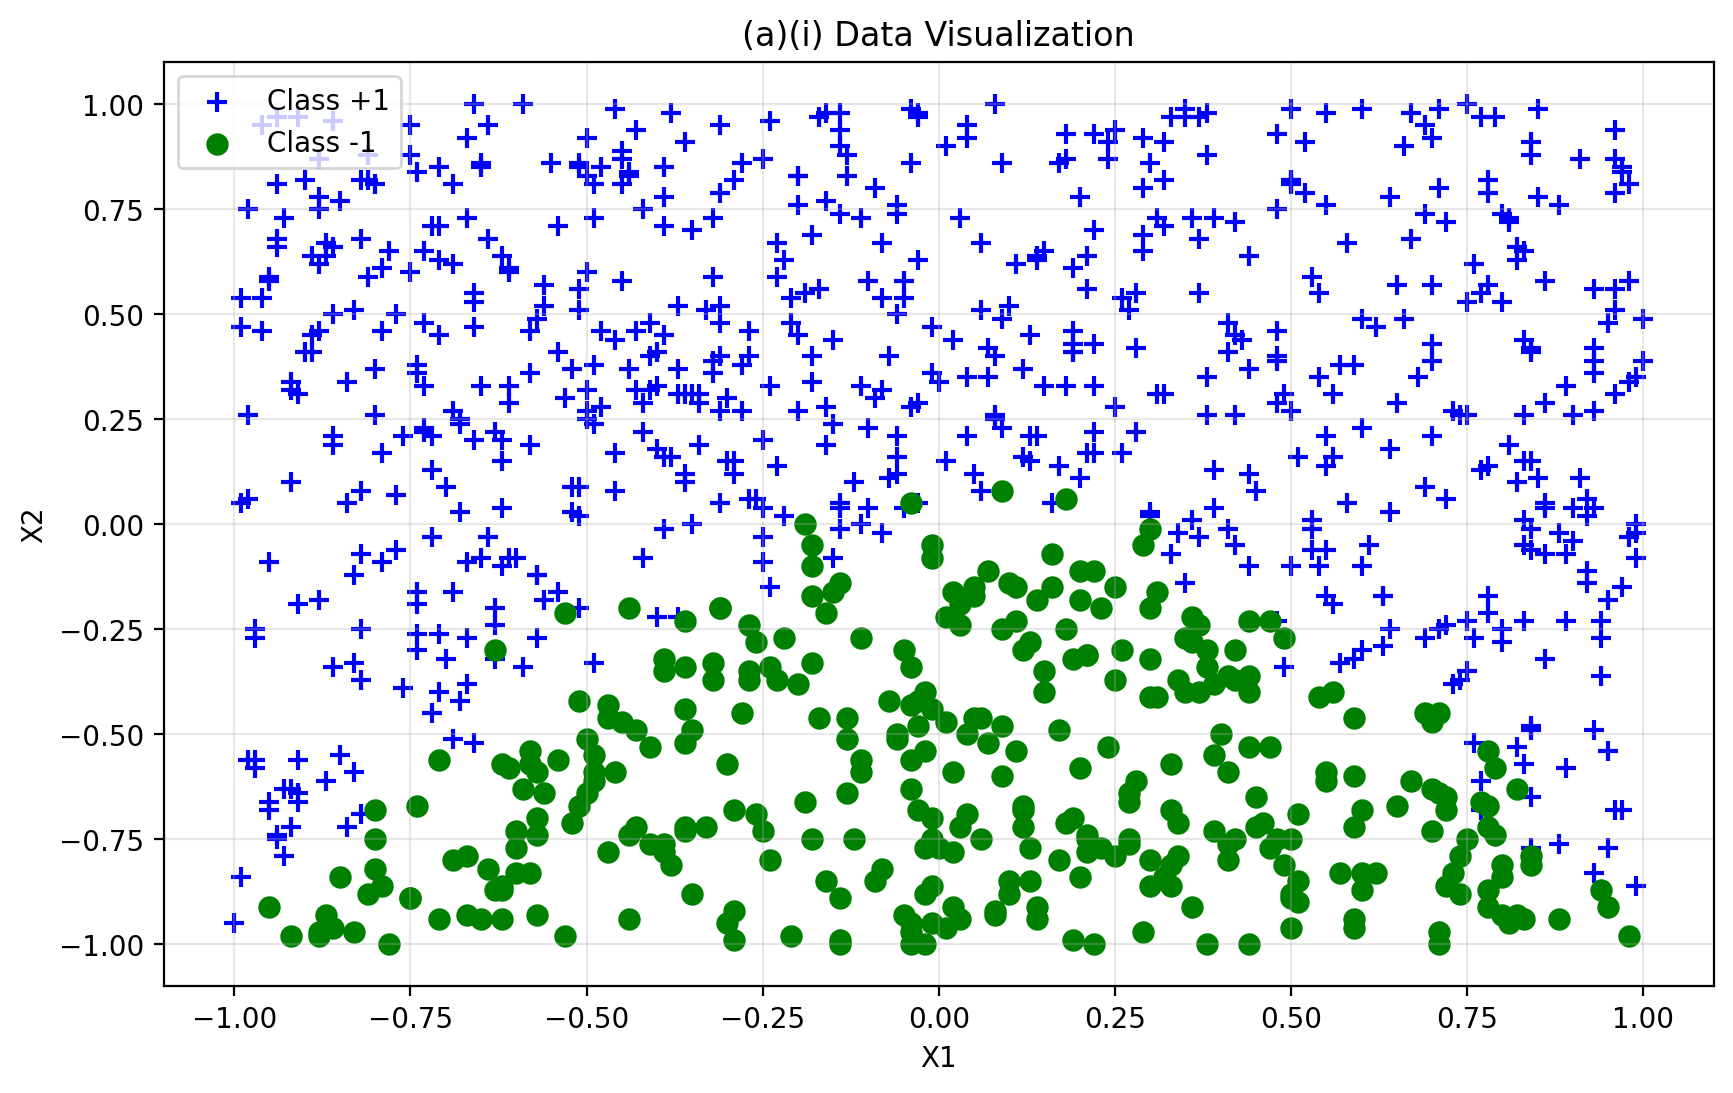
\includegraphics[width=0.7\linewidth]{data_scatter.png}
    \caption{Data visualization: scatter of training data in the \(X_1\)-\(X_2\) plane.}
    \label{fig:data_scatter}
\end{figure}

\subsection{Logistic Regression Model and Parameters}

A logistic regression classifier was trained using scikit-learn's \texttt{LogisticRegression} function, which follows the standard formula:
h(x) = sign($\theta_0 + \theta_1 x_1 + \theta_2 x_2$), where $\theta$ represents the learned parameters

\begin{lstlisting}[language=Python, caption={Model training and parameters extraction}]
logistic_model = LogisticRegression()
logistic_model.fit(X_train, y_train)
w1, w2 = logistic_model.coef_[0]
b = logistic_model.intercept_[0]
\end{lstlisting}

The trained parameters from a representative run were $\theta_0$ (intercept) = 1.7617, $\theta_1$ (X1 coefficient) = -0.2828, and $\theta_2$ (X2 coefficient) = 4.9906. The feature influence analysis reveals that X1 has negative influence since $\theta_1$ = -0.2828 $<$ 0, meaning higher X1 values tend to predict class -1. X2 has positive influence since $\theta_2$ = 4.9906 $>$ 0, meaning higher X2 values tend to predict class +1. X2 is the most influential feature since $|4.9906| > |0.2828|$.

We observe that X2 is the primary determinant of the classification decision because the model puts much more weight on X2 than on X1. From the negative coefficient for X1 we can see that as X1 increases, the model is more likely to predict class -1 while the large positive coefficient for X2 indicates that bigger the X2 values grow, it would strongly favor class +1 predictions.

\subsection{Predictions and Decision Boundary}

I used a trained logistic regression classifier to predict the target values on the training data. I plotted both the predictions along with the actual training data. The decision boundary is derived from the model parameters using the equation $\theta_1 x_1 + \theta_2 x_2 + \theta_0 = 0$, which can be rearranged as $x_2 = -(\theta_1 x_1 + \theta_0)/\theta_2$.

\begin{lstlisting}[language=Python, caption={Decision boundary plotting}]
y_pred_train = logistic_model.predict(X_train)

plt.figure(figsize=(10, 6))
# Plot actual training data
plt.scatter(X_train[y_train==1][:,0], X_train[y_train==1][:,1], 
           marker='+', color='blue', s=50, label="Actual +1")
plt.scatter(X_train[y_train==-1][:,0], X_train[y_train==-1][:,1], 
           marker='o', color='green', s=50, label="Actual -1")

# Plot predictions
plt.scatter(X_train[y_pred_train==1][:,0], X_train[y_pred_train==1][:,1], 
           marker='x', color='cyan', s=50, label="Predicted +1")
plt.scatter(X_train[y_pred_train==-1][:,0], X_train[y_pred_train==-1][:,1], 
           marker='s', color='orange', s=50, label="Predicted -1")

# Decision boundary: w1*x1 + w2*x2 + b = 0 => x2 = -(w1*x1 + b)/w2
x_min, x_max = X_train[:,0].min(), X_train[:,0].max()
y_min_boundary = -(w1*x_min + b)/w2
y_max_boundary = -(w1*x_max + b)/w2

plt.plot([x_min, x_max], [y_min_boundary, y_max_boundary], 
         color='red', linewidth=2, label="Decision Boundary")
\end{lstlisting}

The visualization shows actual training data (blue '+', green 'o'), model predictions (cyan 'x', orange 's'), and the decision boundary (red line). Points above the line are predicted as class +1, below as class -1. The boundary effectively separates most data points with some misclassifications near the boundary.

\begin{figure}[H]
    \centering
    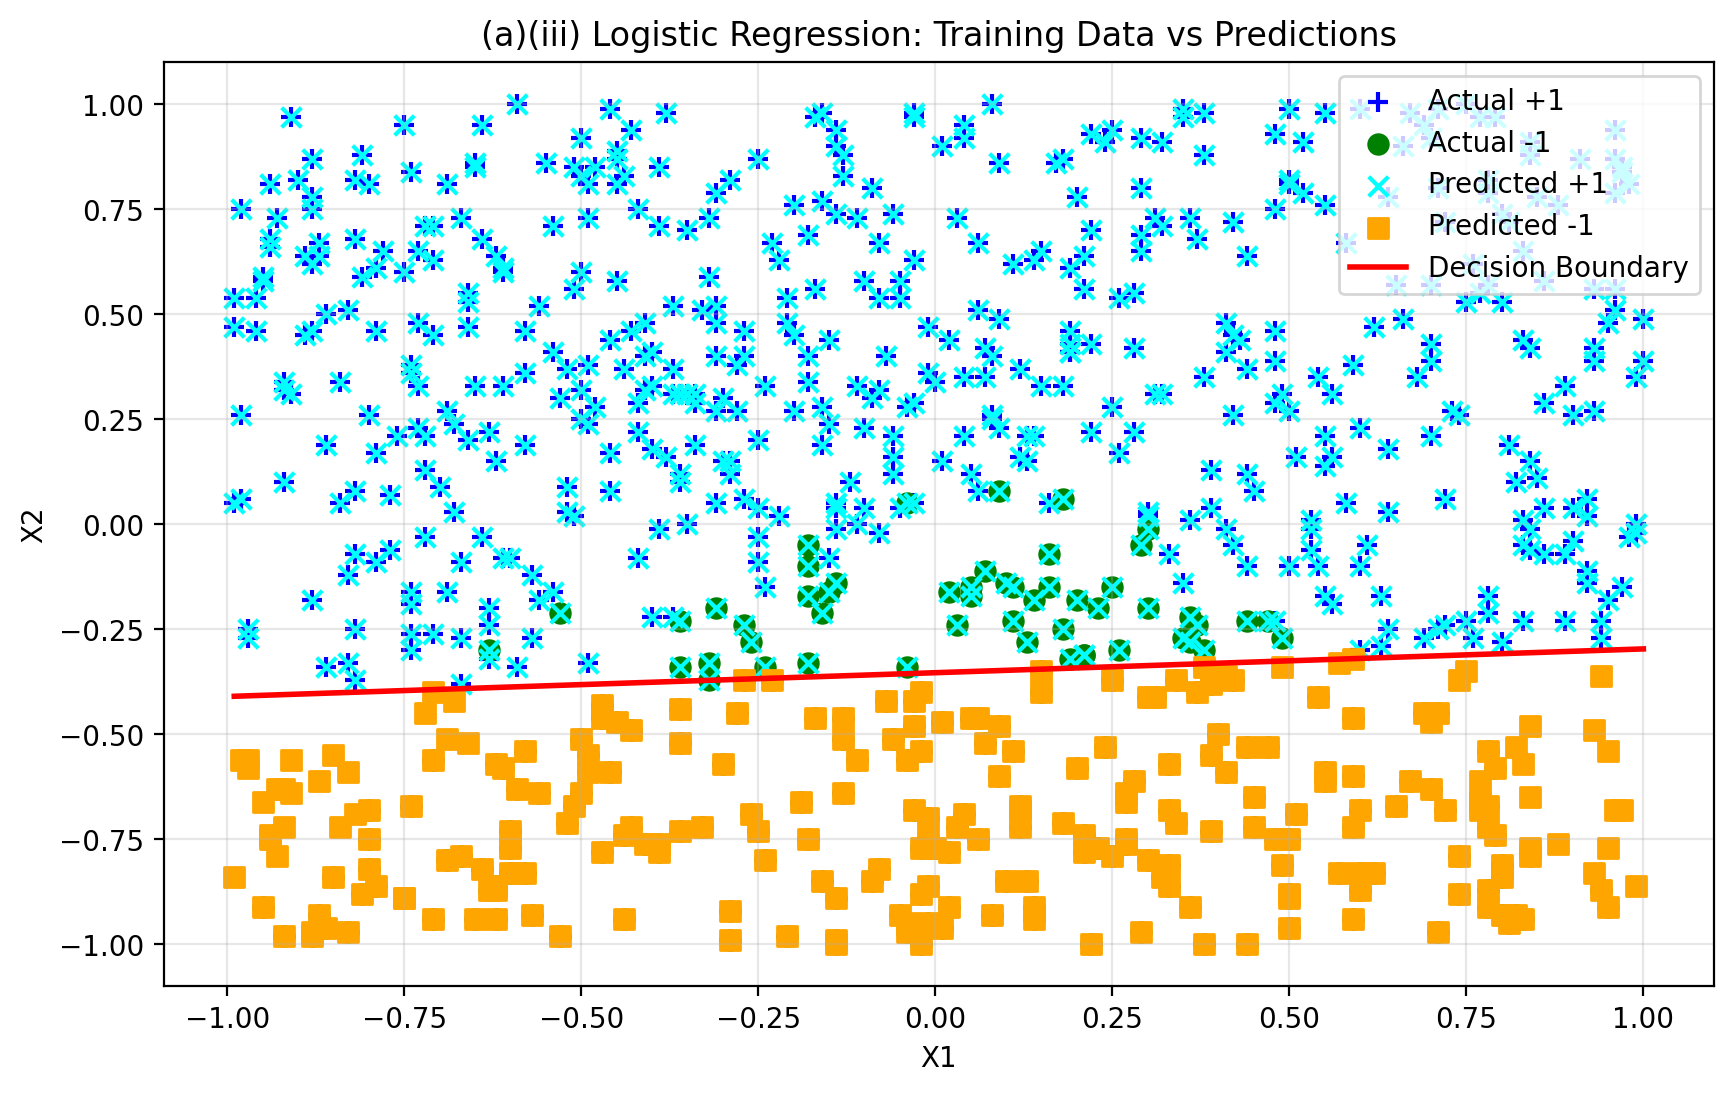
\includegraphics[width=0.7\linewidth]{logistic_boundary.png}
    \caption{Logistic regression: training data, predictions, and linear decision boundary.}
    \label{fig:logistic_boundary}
\end{figure}

\subsection{Comparison of Predictions and Training Data}

After calculating the training accuracy on how well the model performs on the training data, I realised the logistic regression model achieves a representative accuracy of 87.9\% (values vary slightly by train-test split).

\begin{lstlisting}[language=Python, caption={Training Accuracy}]
train_accuracy = accuracy_score(y_train, y_pred_train)
\end{lstlisting}

The model correctly classifies most training samples with few misclassified points near the decision boundary. The high accuracy (87.9\%) demonstrates good performance and indicates the data is largely linearly separable.

\section{Linear SVM}

\subsection{SVM Models with Different C Values}

I trained a SVM classifiers (Linear SVC) using scikit-learn's \texttt{LinearSVC} function for a wide range of C values (C = 0.001, C = 1, and C = 100). The C parameter was used to controls the trade off between margin maximization and classification accuracy in the SVM cost function.

\begin{lstlisting}[language=Python, caption={Training Linear SVM Models}]
from sklearn.svm import LinearSVC
C_values = [0.001, 1, 100]
svm_models = {}
for C in C_values:
    model = LinearSVC(C=C, max_iter=10000)
    model.fit(X_train, y_train)
    svm_models[C] = model

    w1_svm, w2_svm = model.coef_[0]
    b_svm = model.intercept_[0]
\end{lstlisting}

I got different parameter values for each C value. When C was 0.001, the model was h(x) = sign(0.2110 + (-0.0252)*$x_1$ + 0.4169*$x_2$) with weights $w_1$ = -0.0252, $w_2$ = 0.4169, and bias = 0.2110. For C = 1, the model was h(x) = sign(0.6348 + (-0.0877)*$x_1$ + 1.8448*$x_2$) with weights $w_1$ = -0.0877, $w_2$ = 1.8448, and bias = 0.6348. Lastly when C was 100, the model was h(x) = sign(0.6448 + (-0.0893)*$x_1$ + 1.8702*$x_2$) with weights $w_1$ = -0.0893, $w_2$ = 1.8702, and bias = 0.6448.

\subsection{SVM Predictions and Decision Boundaries}

I used each trained SVM classifier to predict the target values on the training data and plotted these predictions along with the actual target values and the classifier decision boundary. Each SVM model with different C values produces different decision boundaries.

\begin{lstlisting}[language=Python, caption={SVM Predictions and Decision Boundaries}]
for C, model in svm_models.items():
    y_pred_svm = model.predict(X_train)
    w1_svm, w2_svm = model.coef_[0]
    b_svm = model.intercept_[0]
    
    plt.figure(figsize=(10, 6))
    
    # Plot actual data
    plt.scatter(X_train[y_train==1][:,0], X_train[y_train==1][:,1], 
               marker='+', color='blue', s=50, label="Actual +1")
    plt.scatter(X_train[y_train==-1][:,0], X_train[y_train==-1][:,1], 
               marker='o', color='green', s=50, label="Actual -1")
    
    # Plot predictions
    plt.scatter(X_train[y_pred_svm==1][:,0], X_train[y_pred_svm==1][:,1], 
               marker='x', color='cyan', s=50, label="Predicted +1")
    plt.scatter(X_train[y_pred_svm==-1][:,0], X_train[y_pred_svm==-1][:,1], 
               marker='s', color='orange', s=50, label="Predicted -1")
    
    # Decision boundary
    x_min, x_max = X_train[:,0].min(), X_train[:,0].max()
    y_min_boundary = -(w1_svm*x_min + b_svm)/w2_svm
    y_max_boundary = -(w1_svm*x_max + b_svm)/w2_svm
    
    plt.plot([x_min, x_max], [y_min_boundary, y_max_boundary], 
             color='red', linewidth=2, label="Decision Boundary")
\end{lstlisting}

C=0.001 creates wider margins prioritizing margin maximization. C=1 provides balanced margin and accuracy. C=100 creates narrower margins prioritizing classification accuracy, potentially leading to overfitting.

\begin{figure}[H]
    \centering
    \includegraphics[width=0.7\linewidth]{svm_c_0001.png}
    \caption{Linear SVM with \(C=0.001\): wider margin, simpler boundary.}
    \label{fig:svm_c_0001}
\end{figure}

\begin{figure}[H]
    \centering
    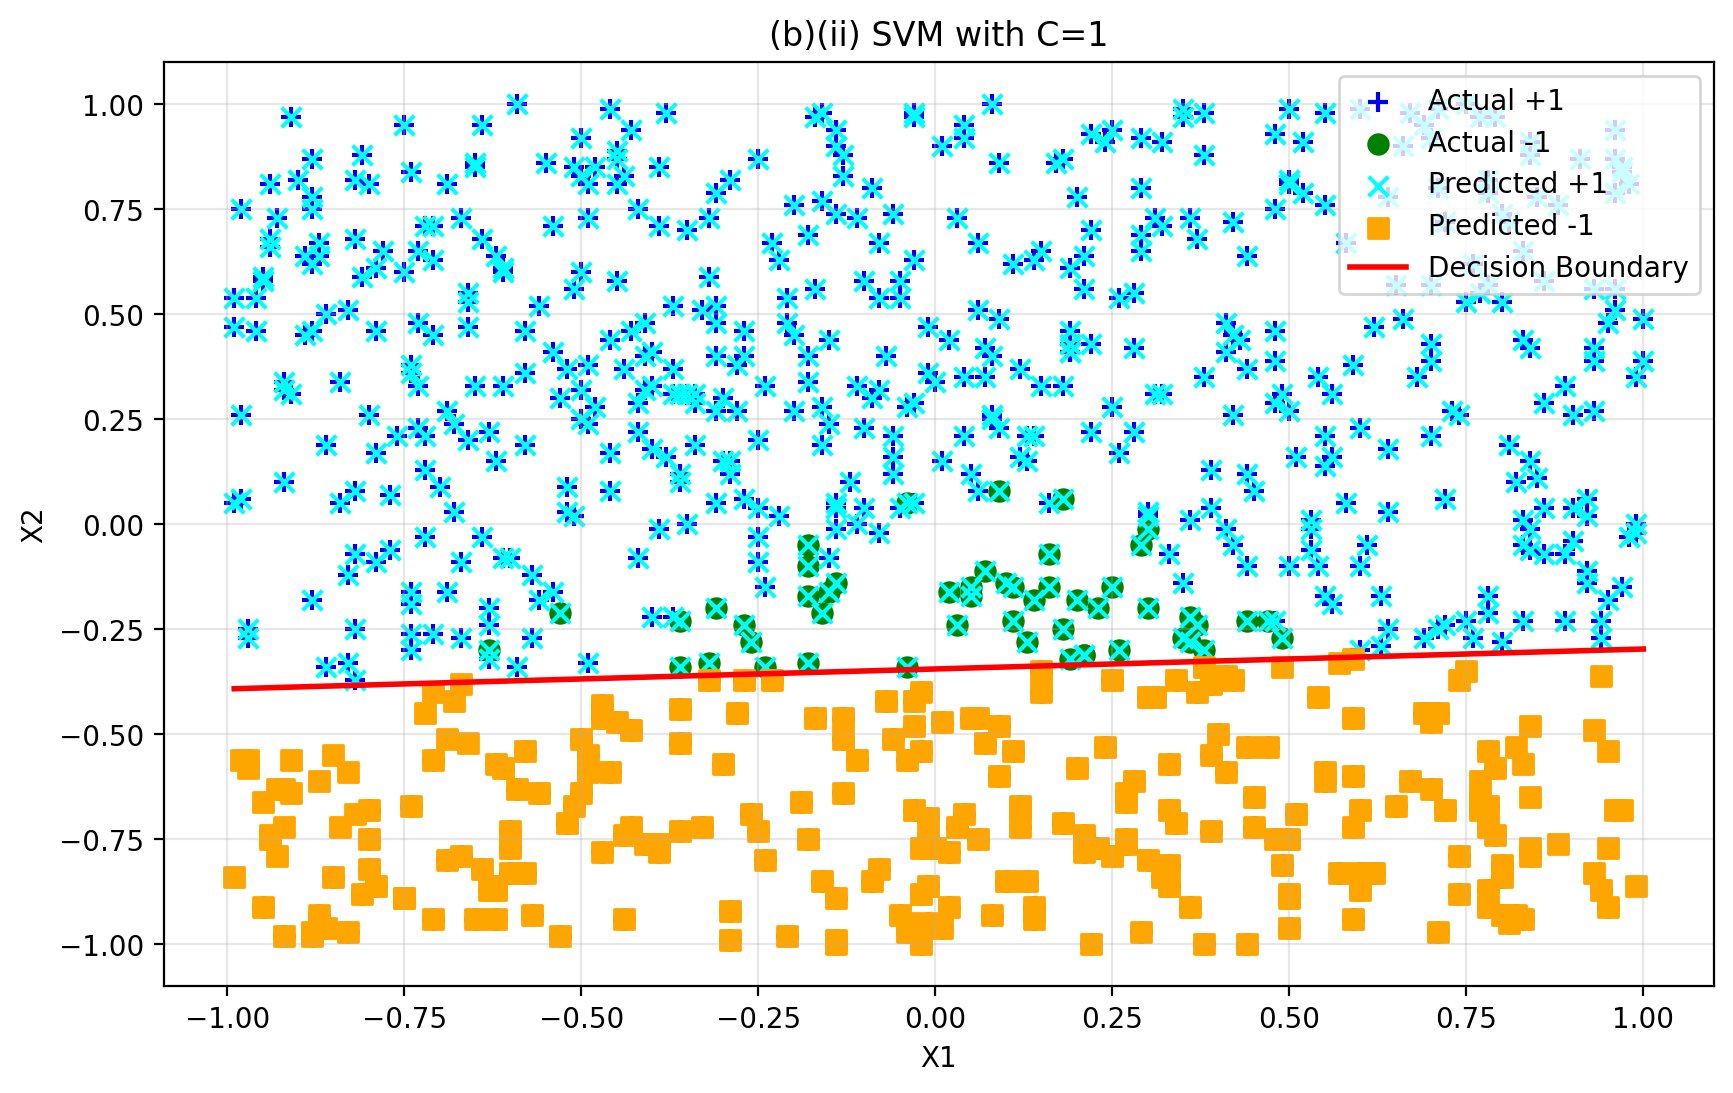
\includegraphics[width=0.7\linewidth]{svm_c_1.png}
    \caption{Linear SVM with \(C=1\): balanced margin and fit.}
    \label{fig:svm_c_1}
\end{figure}

\begin{figure}[H]
    \centering
    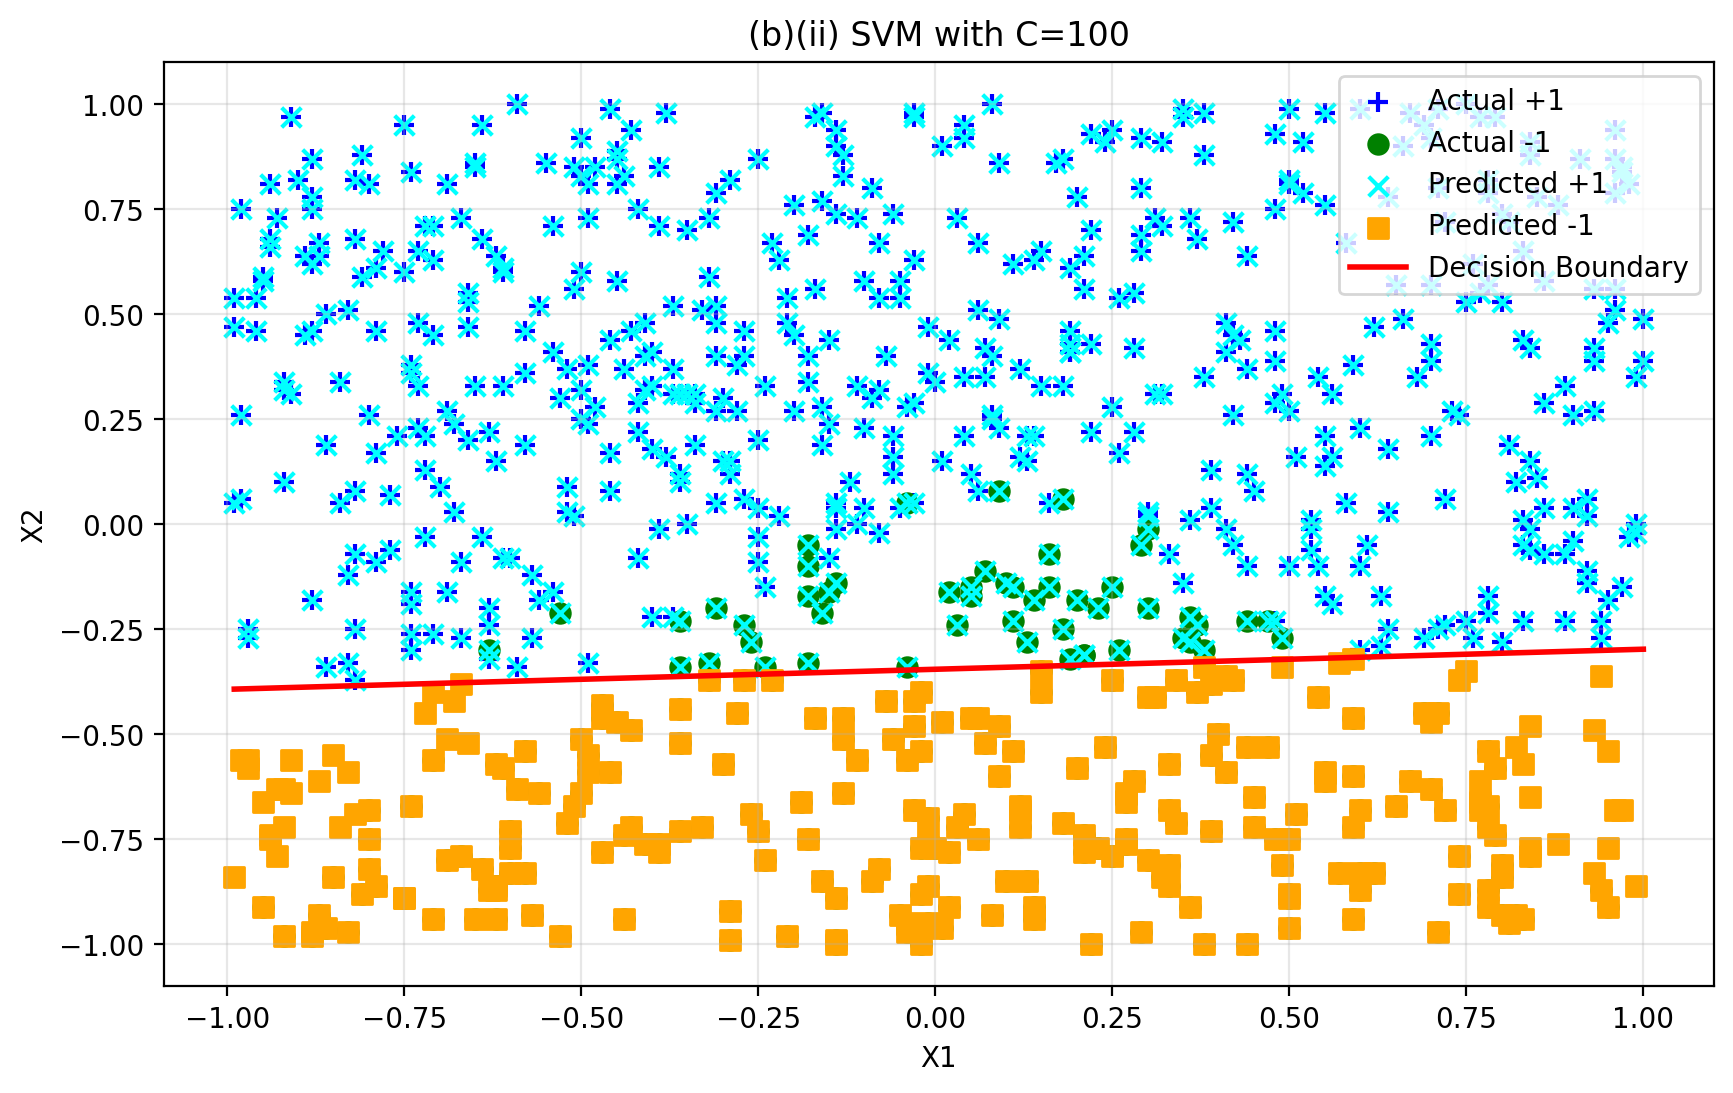
\includegraphics[width=0.7\linewidth]{svm_c_100.png}
    \caption{Linear SVM with \(C=100\): narrower margin, higher complexity.}
    \label{fig:svm_c_100}
\end{figure}

\subsection{Impact of C Parameter}

I analyzed the impact of the C parameter on the model parameters and predictions. The C parameter controls the trade-off in the SVM cost function $J(\theta) = (1/m)\sum\max(0,1-y\theta^T x) + \theta^T\theta/C$.

\begin{lstlisting}[language=Python, caption={Impact of C parameter analysis}]
print(f"\n(b)(iii) Impact of C Parameter:")
for C, model in svm_models.items():
    w1_svm, w2_svm = model.coef_[0]
    b_svm = model.intercept_[0]
    weight_magnitude = np.sqrt(w1_svm**2 + w2_svm**2)
    margin = 1 / weight_magnitude
\end{lstlisting}

Large C (100) results in heavy misclassification penalty, narrower margins, and potential overfitting. Small C (0.001) allows wider margins and better generalization. C=1 provides balanced complexity and generalization.

A larger C makes the penalty term $\theta^T\theta/C$ smaller, allowing the model to use larger weights to minimize misclassifications. A smaller C makes the penalty term larger, encouraging the model to use smaller weights and prioritize margin maximization.

\subsection{SVM vs Logistic Regression Comparison}

I compared the SVM model parameters and predictions with those of the logistic regression model. Both models achieve comparable accuracy, indicating that both approaches are effective for this dataset.

\begin{lstlisting}[language=Python, caption={SVM vs Logistic Regression comparison}]
svm_model_c1 = svm_models[1]
w1_svm, w2_svm = svm_model_c1.coef_[0]
b_svm = svm_model_c1.intercept_[0]
svm_accuracy = accuracy_score(y_train, svm_model_c1.predict(X_train))
\end{lstlisting}

The logistic regression model had weights $w_1$ = -0.2828, $w_2$ = 4.9906, bias = 1.7617, and training accuracy of 87.9\%. The SVM (C = 1) model had weights $w_1$ = -0.0877, $w_2$ = 1.8448, bias = 0.6348, and training accuracy of 87.9\%. SVM weights are generally smaller than logistic regression weights due to the regularization term $\theta^T\theta/C$ in the SVM cost function, this regularization in turn encouraged the SVM to find a solution with smaller weights.

Both models produce linear decision boundaries. SVM focuses on margin maximization using hinge loss and support vectors, while logistic regression uses logistic loss and considers all points. SVM is more robust to outliers.

\section{Polynomial Features}

\subsection{Extended Feature Set}

I created two additional features by adding the square of each original feature, giving four features in total: $X_1$, $X_2$, $X_1^2$, and $X_2^2$. I then trained a logistic regression classifier on this extended feature set.

\begin{lstlisting}[language=Python, caption={Extended Feature Set}]
X1_squared = X1**2
X2_squared = X2**2
X_extended = np.column_stack((X1, X2, X1_squared, X2_squared))
poly_model = LogisticRegression()
poly_model.fit(X_extended, y)

w1_poly, w2_poly, w3_poly, w4_poly = poly_model.coef_[0]
b_poly = poly_model.intercept_[0]
\end{lstlisting}

The extended model is h(x) = sign($\theta_0 + \theta_1 x_1 + \theta_2 x_2 + \theta_3 x_1^2 + \theta_4 x_2^2$). The trained parameters were $\theta_0$ (intercept) = 0.4174, $\theta_1$ ($X_1$ coefficient) = -0.3720, $\theta_2$ ($X_2$ coefficient) = 6.8509, $\theta_3$ ($X_1^2$ coefficient) = 6.6088, and $\theta_4$ ($X_2^2$ coefficient) = -1.1069. The complete model equation is h(x) = sign(0.4174 + (-0.3720)*$x_1$ + 6.8509*$x_2$ + 6.6088*$x_1^2$ + (-1.1069)*$x_2^2$).

\subsection{Predictions and Comparison}

I used the trained polynomial logistic regression classifier to predict the target values on the training data and compared the performance with the previous linear models.

\begin{lstlisting}[language=Python, caption={Predictions and comparison}]
y_pred_poly = poly_model.predict(X_extended)
poly_accuracy = accuracy_score(y, y_pred_poly)

plt.figure(figsize=(10, 6))
# Plot actual data
plt.scatter(X1[y==1], X2[y==1], marker='+', color='blue', s=50, label="Actual +1")
plt.scatter(X1[y==-1], X2[y==-1], marker='o', color='green', s=50, label="Actual -1")

# Plot predictions
plt.scatter(X1[y_pred_poly==1], X2[y_pred_poly==1], marker='x', color='cyan', s=50, label="Predicted +1")
plt.scatter(X1[y_pred_poly==-1], X2[y_pred_poly==-1], marker='s', color='orange', s=50, label="Predicted -1")
\end{lstlisting}

\begin{figure}[H]
    \centering
    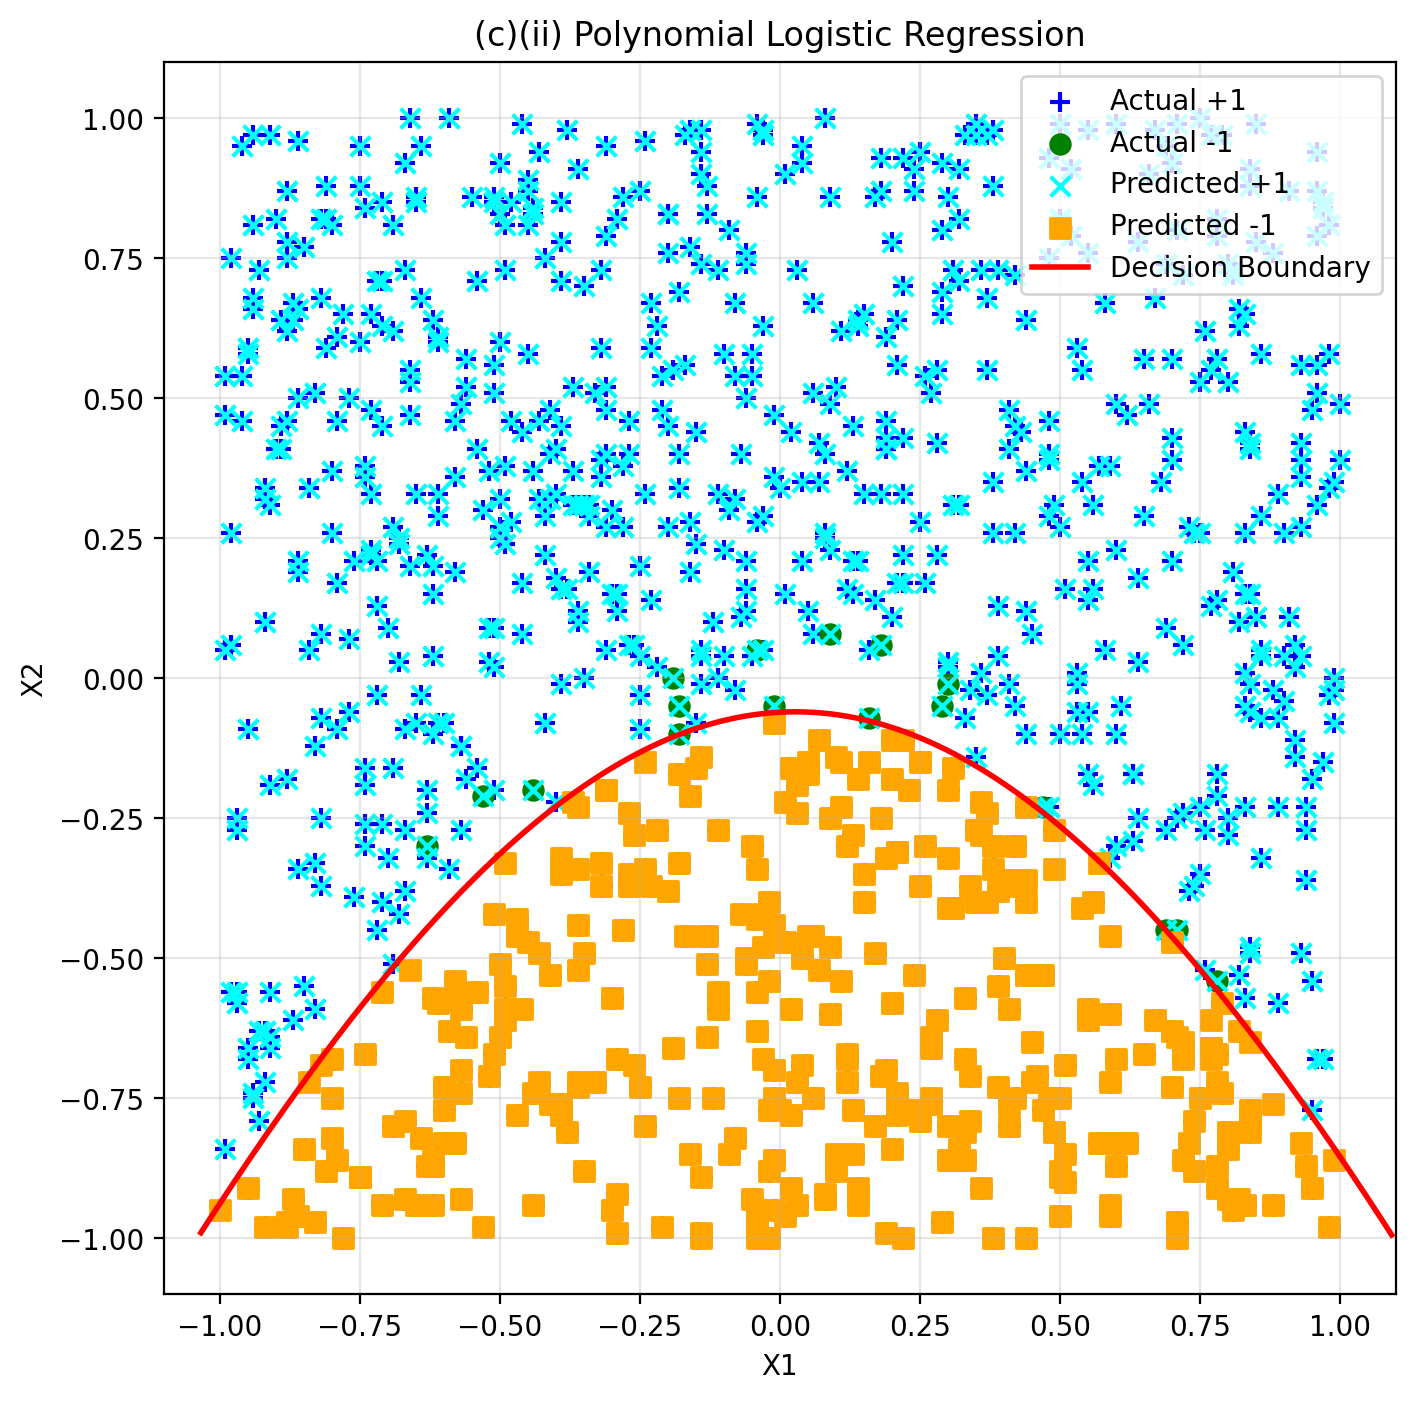
\includegraphics[width=0.7\linewidth]{poly_boundary.png}
    \caption{Polynomial logistic regression: quadratic decision boundary with data and predictions.}
    \label{fig:poly_boundary}
\end{figure}

Polynomial features achieve 96.6\% accuracy vs 87.9\% (logistic) and 87.9\% (SVM), demonstrating non-linear relationships. The quadratic decision boundary better separates classes in regions where linear boundaries are less effective.

Including $X_1^2$ and $X_2^2$ terms helps the model to catch quadratic relationships of the form. The positive coefficient of $X_1^2$ supports the idea that $X_1$ has a quadratic feature of relationships in the target variable while the negative coefficient of $X_2^2$ will demonstrate some other quadratic patterns of relationships for $X_2$.

\subsection{Baseline Comparison}

I compared the performance of the polynomial classifier against a reasonable baseline predictor that always predicts the most common class.

\begin{lstlisting}[language=Python, caption={Baseline comparison}]
most_common_class = np.bincount(y + 1).argmax() - 1  # Convert -1,1 to 0,2 then back
baseline_accuracy = np.mean(y == most_common_class)
\end{lstlisting}

The baseline predictor (always predicting the most common class) achieves 65.6\% accuracy. All ML models significantly outperform: logistic regression (87.9\%), SVM (87.9\%), and polynomial logistic regression (96.6\%). Polynomial features show 31.0\% improvement over baseline by capturing non-linear patterns.

\subsection{Quadratic Decision Boundary (Bonus)}

I plotted the classifier decision boundary, which is no longer a straight line but a quadratic curve. The decision boundary equation is $\theta_1 x_1 + \theta_2 x_2 + \theta_3 x_1^2 + \theta_4 x_2^2 + \theta_0 = 0$. Rearranging the same to solve for $x_2$: $\theta_4 x_2^2 + \theta_2 x_2 + (\theta_1 x_1 + \theta_3 x_1^2 + \theta_0) = 0$.

\begin{lstlisting}[language=Python, caption={Quadratic decision boundary}]
# Quadratic decision boundary
x_vals = np.linspace(-1, 1, 300)
y_boundary_pos = []
y_boundary_neg = []

for x in x_vals:
    # Quadratic equation: w2*x2 + w4*x2² + w1*x1 + w3*x1² + b = 0
    A = w4_poly
    B = w2_poly
    C = w1_poly*x + w3_poly*x**2 + b_poly
    
    discriminant = B**2 - 4*A*C
    if discriminant >= 0:
        sqrt_disc = np.sqrt(discriminant)
        y_boundary_pos.append((-B + sqrt_disc)/(2*A))
        y_boundary_neg.append((-B - sqrt_disc)/(2*A))
    else:
        y_boundary_pos.append(np.nan)
        y_boundary_neg.append(np.nan)

# Filter boundaries to be within the plot range
y_boundary_pos = [y if -1 <= y <= 1 else np.nan for y in y_boundary_pos]
y_boundary_neg = [y if -1 <= y <= 1 else np.nan for y in y_boundary_neg]

# Plot decision boundary
plt.plot(x_vals, y_boundary_pos, color='red', linewidth=2, label="Decision Boundary")
plt.plot(x_vals, y_boundary_neg, color='red', linewidth=2)

plt.xlabel("X1")
plt.ylabel("X2")
plt.title("(c)(ii) Polynomial Logistic Regression")
plt.xlim(-1, 1)
plt.ylim(-1, 1)
plt.legend()
plt.grid(True, alpha=0.3)
plt.show()
\end{lstlisting}

This represents a quadratic equation $ax_2^2 + bx_2 + c = 0$ where $a = \theta_4 = -1.1069$, $b = \theta_2 = 6.8509$, and $c = \theta_1 x_1 + \theta_3 x_1^2 + \theta_0$. The solution $x_2 = (-b \pm \sqrt{b^2 - 4ac}) / 2a$ creates a curved decision boundary enabling non-linear class separation and improved accuracy.

\section*{APPENDIX}

\begin{lstlisting}[language=Python]
import numpy as np
import pandas as pd
import matplotlib.pyplot as plt
from sklearn.linear_model import LogisticRegression
from sklearn.model_selection import train_test_split
from sklearn.metrics import accuracy_score

# Load dataset
df = pd.read_csv("week2.csv", skiprows=1, header=None)
df.columns = ["X1", "X2", "y"]

# Extract features and target
X1 = df["X1"].values
X2 = df["X2"].values
y = df["y"].values
X = np.column_stack((X1, X2))

# (a)(i) Data visualization
plt.figure(figsize=(10, 6))
plt.scatter(X1[y==1], X2[y==1], marker='+', color='blue', s=50, label="Class +1")
plt.scatter(X1[y==-1], X2[y==-1], marker='o', color='green', s=50, label="Class -1")
plt.xlabel("X1")
plt.ylabel("X2")
plt.title("(a)(i) Data Visualization")
plt.legend()
plt.grid(True, alpha=0.3)
plt.show()

# Train-test split
X_train, X_test, y_train, y_test = train_test_split(X, y, test_size=0.2, random_state=42)

# (a)(ii) Train logistic regression
logistic_model = LogisticRegression()
logistic_model.fit(X_train, y_train)

# Extract parameters
w1, w2 = logistic_model.coef_[0]
b = logistic_model.intercept_[0]

# (a)(iii) Predictions on training data
y_pred_train = logistic_model.predict(X_train)

plt.figure(figsize=(10, 6))
plt.scatter(X_train[y_train==1][:,0], X_train[y_train==1][:,1], 
           marker='+', color='blue', s=50, label="Actual +1")
plt.scatter(X_train[y_train==-1][:,0], X_train[y_train==-1][:,1], 
           marker='o', color='green', s=50, label="Actual -1")
plt.scatter(X_train[y_pred_train==1][:,0], X_train[y_pred_train==1][:,1], 
           marker='x', color='cyan', s=50, label="Predicted +1")
plt.scatter(X_train[y_pred_train==-1][:,0], X_train[y_pred_train==-1][:,1], 
           marker='s', color='orange', s=50, label="Predicted -1")

x_min, x_max = X_train[:,0].min(), X_train[:,0].max()
y_min_boundary = -(w1*x_min + b)/w2
y_max_boundary = -(w1*x_max + b)/w2
plt.plot([x_min, x_max], [y_min_boundary, y_max_boundary], 
         color='red', linewidth=2, label="Decision Boundary")

plt.xlabel("X1")
plt.ylabel("X2")
plt.title("(a)(iii) Logistic Regression: Training Data vs Predictions")
plt.legend()
plt.grid(True, alpha=0.3)
plt.show()

# (a)(iv) Training accuracy
train_accuracy = accuracy_score(y_train, y_pred_train)
# (b)(i) Train SVM with different C values
from sklearn.svm import LinearSVC
C_values = [0.001, 1, 100]
svm_models = {}

for C in C_values:
    model = LinearSVC(C=C, max_iter=10000)
    model.fit(X_train, y_train)
    svm_models[C] = model

# (b)(ii) Plot SVM results
for C, model in svm_models.items():
    y_pred_svm = model.predict(X_train)
    w1_svm, w2_svm = model.coef_[0]
    b_svm = model.intercept_[0]
    
    plt.figure(figsize=(10, 6))
    
    # Plot actual data
    plt.scatter(X_train[y_train==1][:,0], X_train[y_train==1][:,1], 
               marker='+', color='blue', s=50, label="Actual +1")
    plt.scatter(X_train[y_train==-1][:,0], X_train[y_train==-1][:,1], 
               marker='o', color='green', s=50, label="Actual -1")
    
    # Plot predictions
    plt.scatter(X_train[y_pred_svm==1][:,0], X_train[y_pred_svm==1][:,1], 
               marker='x', color='cyan', s=50, label="Predicted +1")
    plt.scatter(X_train[y_pred_svm==-1][:,0], X_train[y_pred_svm==-1][:,1], 
               marker='s', color='orange', s=50, label="Predicted -1")
    
    # Decision boundary
    x_min, x_max = X_train[:,0].min(), X_train[:,0].max()
    y_min_boundary = -(w1_svm*x_min + b_svm)/w2_svm
    y_max_boundary = -(w1_svm*x_max + b_svm)/w2_svm
    
    plt.plot([x_min, x_max], [y_min_boundary, y_max_boundary], 
             color='red', linewidth=2, label="Decision Boundary")
    
    plt.xlabel("X1")
    plt.ylabel("X2")
    plt.title(f"(b)(ii) SVM with C={C}")
    plt.legend()
    plt.grid(True, alpha=0.3)
    plt.show()

# (c)(i) Create polynomial features
X1_squared = X1**2
X2_squared = X2**2
X_extended = np.column_stack((X1, X2, X1_squared, X2_squared))

# Train logistic regression with extended features
poly_model = LogisticRegression()
poly_model.fit(X_extended, y)

# Extract parameters
w1_poly, w2_poly, w3_poly, w4_poly = poly_model.coef_[0]
b_poly = poly_model.intercept_[0]

# (c)(ii) Predictions and comparison
y_pred_poly = poly_model.predict(X_extended)
poly_accuracy = accuracy_score(y, y_pred_poly)

plt.figure(figsize=(10, 6))
plt.scatter(X1[y==1], X2[y==1], marker='+', color='blue', s=50, label="Actual +1")
plt.scatter(X1[y==-1], X2[y==-1], marker='o', color='green', s=50, label="Actual -1")
plt.scatter(X1[y_pred_poly==1], X2[y_pred_poly==1], marker='x', color='cyan', s=50, label="Predicted +1")
plt.scatter(X1[y_pred_poly==-1], X2[y_pred_poly==-1], marker='s', color='orange', s=50, label="Predicted -1")

# Quadratic decision boundary
x_vals = np.linspace(-1, 1, 300)
y_boundary_pos = []
y_boundary_neg = []

for x in x_vals:
    A = w4_poly
    B = w2_poly
    C = w1_poly*x + w3_poly*x**2 + b_poly
    
    discriminant = B**2 - 4*A*C
    if discriminant >= 0:
        sqrt_disc = np.sqrt(discriminant)
        y_boundary_pos.append((-B + sqrt_disc)/(2*A))
        y_boundary_neg.append((-B - sqrt_disc)/(2*A))
    else:
        y_boundary_pos.append(np.nan)
        y_boundary_neg.append(np.nan)

y_boundary_pos = [y if -1 <= y <= 1 else np.nan for y in y_boundary_pos]
y_boundary_neg = [y if -1 <= y <= 1 else np.nan for y in y_boundary_neg]

plt.plot(x_vals, y_boundary_pos, color='red', linewidth=2, label="Decision Boundary")
plt.plot(x_vals, y_boundary_neg, color='red', linewidth=2)

plt.xlabel("X1")
plt.ylabel("X2")
plt.title("(c)(ii) Polynomial Logistic Regression")
plt.xlim(-1, 1)
plt.ylim(-1, 1)
plt.legend()
plt.grid(True, alpha=0.3)
plt.show()

# (c)(iii) Baseline comparison
most_common_class = np.bincount(y + 1).argmax() - 1  # Convert -1,1 to 0,2 then back
baseline_accuracy = np.mean(y == most_common_class)

# (c)(iv) Bonus: Quadratic Decision Boundary

plt.figure(figsize=(8, 8))
# Plot actual and predicted points
plt.scatter(X1[y==1], X2[y==1], marker='+', color='blue', label="Actual +1", alpha=0.7)
plt.scatter(X1[y==-1], X2[y==-1], marker='o', color='green', label="Actual -1", alpha=0.7)
plt.scatter(X1[y_pred_poly==1], X2[y_pred_poly==1], marker='x', color='cyan', label="Predicted +1", alpha=0.6)
plt.scatter(X1[y_pred_poly==-1], X2[y_pred_poly==-1], marker='s', color='orange', label="Predicted -1", alpha=0.6)

x_vals = np.linspace(X1.min()-1, X1.max()+1, 300)
y_boundary_pos = []
y_boundary_neg = []

for x in x_vals:
    A = w4_poly
    B = w2_poly
    C = w1_poly*x + w3_poly*x**2 + b_poly

    discriminant = B**2 - 4*A*C
    if discriminant >= 0:
        sqrt_disc = np.sqrt(discriminant)
        y_boundary_pos.append((-B + sqrt_disc)/(2*A))
        y_boundary_neg.append((-B - sqrt_disc)/(2*A))
    else:
        y_boundary_pos.append(np.nan)
        y_boundary_neg.append(np.nan)

# Filter boundaries to be within the data range
y_boundary_pos = [y if X2.min()-1 <= y <= X2.max()+1 else np.nan for y in y_boundary_pos]
y_boundary_neg = [y if X2.min()-1 <= y <= X2.max()+1 else np.nan for y in y_boundary_neg]

plt.plot(x_vals, y_boundary_pos, color='red', linewidth=2, label="Decision Boundary")
plt.plot(x_vals, y_boundary_neg, color='red', linewidth=2)

# Make axes proportional and set bounds tightly around data
plt.gca().set_aspect('equal', adjustable='box')
plt.xlim(X1.min()-0.1, X1.max()+0.1)
plt.ylim(X2.min()-0.1, X2.max()+0.1)

plt.xlabel("X1")
plt.ylabel("X2")
plt.title("(c)(iv) Bonus: Quadratic Decision Boundary")
plt.legend()
plt.grid(True, alpha=0.3)
plt.show()

\end{lstlisting}

\end{document}